\documentclass[preview,convert={outext=.svg,command=\unexpanded{pdf2svg \infile\space\outfile}},multi=false]{standalone}[2012/04/13]
\usepackage{tikz}
\usetikzlibrary{arrows, calc}
\usepackage{amsmath}

%% common idioms for diagrams
\def\Hask{\mathsf{Hask}}
\def\Id{\mathsf{Id}}
\def\T{\mathsf{T}}
\def\id{\mathsf{id}}



%% we want a path that gives a double arrow of fixed length
%% strategy: go to the midpoint, go forwards, and backwards by a fixed distance
\def\2cell{}

\begin{document}
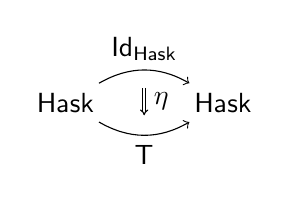
\begin{tikzpicture}[node distance=2cm, auto]
  \node (H1) {$\Hask$};
  \node (H2) [right of= H1] {$\Hask$};
  \draw[->, bend left] (H1) to node (id) [above] {$\Id_{\Hask}$} (H2);
  \draw[->, bend right] (H1) to node (t) [below] {$\T$} (H2);
  \draw[->, double, -implies] ($(id)!5mm!(t)$)  to node[right] {$\eta$} ($(t)!5mm!(id)$);
\end{tikzpicture}
\end{document}